% !TEX root =  ../main_manuscript.tex 
\subsection{Statistical Methods}
Our aim was to develop a model for predicting the time of GS7. The available data for each patient were, age at the start of AS, all observed PSA measurements, and the history of biopsies. We wanted to account for the correlation between the PSA measurements of the same patient, and also their correlation with the time of GS7. An additional complication was that the PSA values were missing once a patient obtained GS7. A commonly used model to handle these issues is the joint model for time-to-event and longitudinal data \citep{rizopoulos2012joint,tomer2019,coley2017prediction}.

\begin{figure}[!htb]
\centerline{\includegraphics[width=\columnwidth]{images/jm_blockdiag.pdf}}
\caption{\textbf{Diagram of the joint model}: Patient-specific random effects (ellipse in center) are shared between sub-models for all outcomes pertaining to prostate cancer progression. The random effects model the correlation between the outcomes. In the linear mixed effects sub-model for $\log_2\{\mbox{PSA + 1}\}$ transformed PSA outcome (bottom rectangle), random effects are used as covariates. In the relative-risk sub-model (similar to Cox model) for time of Gleason~$\geq$~7 (GS7), random effects are utilized indirectly, by including fitted $\log_2\{\mbox{PSA + 1}\}$ value and velocities as covariates. Age of patient at baseline is included in both sub-models. Parameters of both sub-models are estimated jointly.}
\label{fig:jm_blockdiag}
\end{figure}

The joint model we utilized, exploited patient-specific random effects \citep{laird1982random} to act as a common source of correlation between the PSA and time of GS7 outcomes (see Figure~\ref{fig:jm_blockdiag} and Appendix A.2's Figure~1). Random effects also represented the underlying state of PCa, and were included in both the linear mixed effects sub-model for $\log_2\{\mbox{PSA + 1}\}$ transformed measurements (see Appendix A.5), and the relative risk sub-model (similar to cox model) for time of GS7. In the sub-model for PSA, random effects non-linearly modeled the evolution of PSA over time. Simultaneously, in the relative risk model random effects were used indirectly by including fitted $\log_2\{\mbox{PSA + 1}\}$ value and velocity as time dependent covariates. This established the correlation between PSA and time of GS7. Unlike observed $\log_2\{\mbox{PSA + 1}\}$ values, the fitted values were free of measurement errors. The $\log_2\{\mbox{PSA + 1}\}$ velocity was mathematically derived from fitted $\log_2\{\mbox{PSA + 1}\}$ values. Consequently, the $\log_2\{\mbox{PSA + 1}\}$ velocity also changed non-linearly over follow-up.

The parameters of the two sub-models were estimated jointly using the R package \textbf{JMbayes} \citep{rizopoulosJMbayes}. This package utilizes the Bayesian methodology to estimate model parameters.

\subsection{Assessment of Predictions of GS7}
We validated the risk predictions of GS7 from our model within the PRIAS dataset (internal validation), as well as in five of the largest AS cohorts part of the GAP3 database \citep{gap3_2018} (external validation). The external cohorts were University of Toronto AS (Toronto), Johns Hopkins AS (JHAS), Memorial Sloan Kettering Cancer Center AS (MSKCC), King's College London AS (KCL), and Michigan Urological Surgery Improvement Collaborative AS (MUSIC). For validation, we utilized the area under the receiver operating characteristic curve or AUC \cite{rizopoulos2017dynamic} as a measure of discrimination, and root mean squared prediction error or RMSPE \cite{rizopoulos2017dynamic} as a measure of calibration. Since AS studies are longitudinal in nature, we computed AUC and RMSPE in a time dependent manner, at a gap of every six months (follow-up schedule of PRIAS) until year five (95-percentile of the observed GS7 times in PRIAS) of follow-up.

\subsection{Personalized Schedule of Biopsies, and Its Consequences}
Consider a new patient shown in Figure~\ref{fig:demo_pat1} for whom we intended to make a personalized schedule of biopsies. First, using the joint model fitted to the PRIAS dataset we obtained his cumulative risk of GS7 over the entire follow-up period (Panel~B of Figure~\ref{fig:demo_pat1}). A biopsy at his current visit may be then suggested if the cumulative risk of GS7 at the current visit is above a certain threshold (e.g., 10\% risk). By repeatedly applying this 10\% threshold rule over the whole follow-up, we obtained his personalized schedule of biopsies (see Appendix C). Similar schedules can be made with another risk threshold such as 5\% or 15\% risk. These personalized risk based biopsy schedules are updated at each follow-up visit based on newly gathered patient data. 

To assist patients in making an informed choice for a schedule, be it personalized or fixed, we provided them patient-specific consequences of following each schedule. To this end, we first calculated the probability of occurrence of GS7 in time gaps between successive biopsies of each schedule. Using these probabilities we then obtained the expected time delay in detection of GS7 for following that schedule (see Appendix C). Thus, patients had a method to compare across various schedules in terms of the personalized burden (time and total biopsies), and personalized benefit (less delay in detection of GS7 is beneficial). Lastly, we implemented this approach in a web-application.

\begin{figure}[!htb]
\centerline{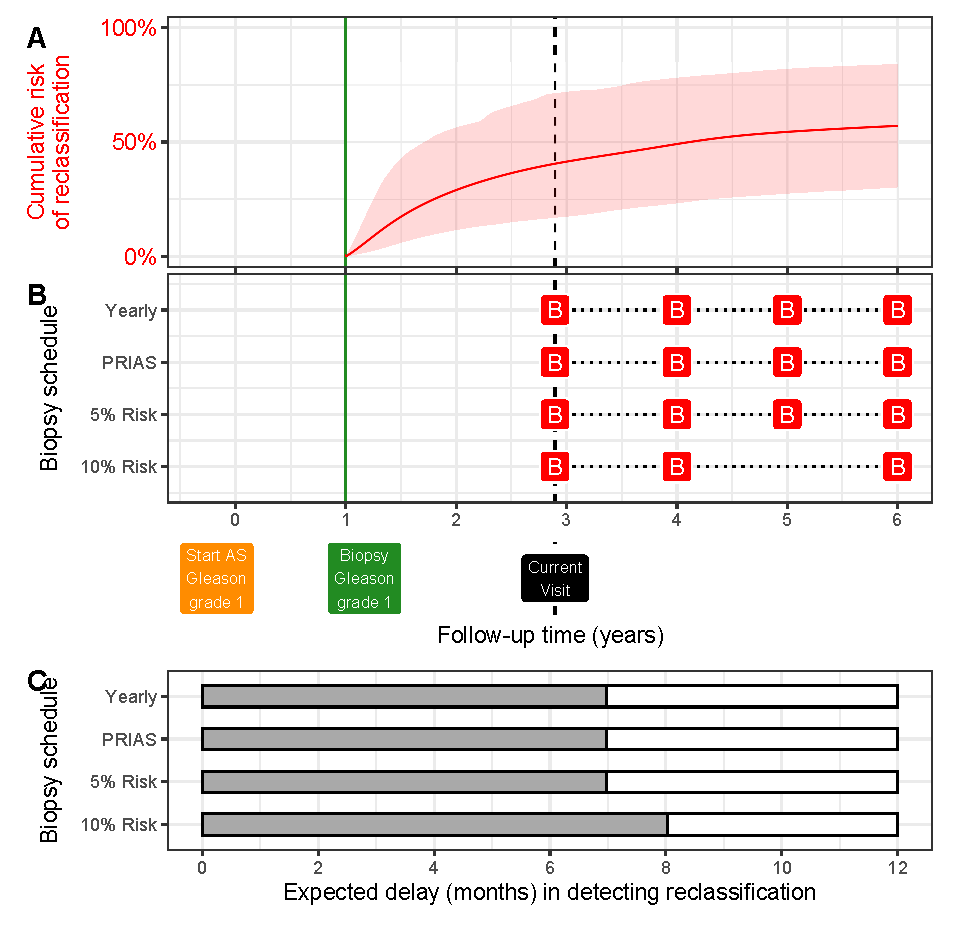
\includegraphics[width=\columnwidth]{images/demo_pat1.eps}}
\caption{\textbf{Personalized and fixed schedules of biopsies for new patient}. \textbf{Panel~A,B:} show the observed and fitted $\log_2(\mbox{PSA} + 1)$ measurements, and the dynamic cumulative risk of Gleason $\geq$ 7 over the follow-up period. \textbf{Panel~C} shows the personalized and fixed schedules of biopsies with a `B' indicating the time of biopsy. In the bottom two panels, the various schedules are compared in terms of the number of biopsies they schedule, and the expected delay in detection of Gleason $\geq$ 7 if they are followed.}
\label{fig:demo_pat1}
\end{figure}